 %!TEX root = ./template-skripsi.tex
%-------------------------------------------------------------------------------
%                            BAB II
%               KAJIAN TEORI
%-------------------------------------------------------------------------------

\chapter{KAJIAN PUSTAKA} 

\section{World Wide Web (WWW)}

\begin{figure}[H]
	\centering
	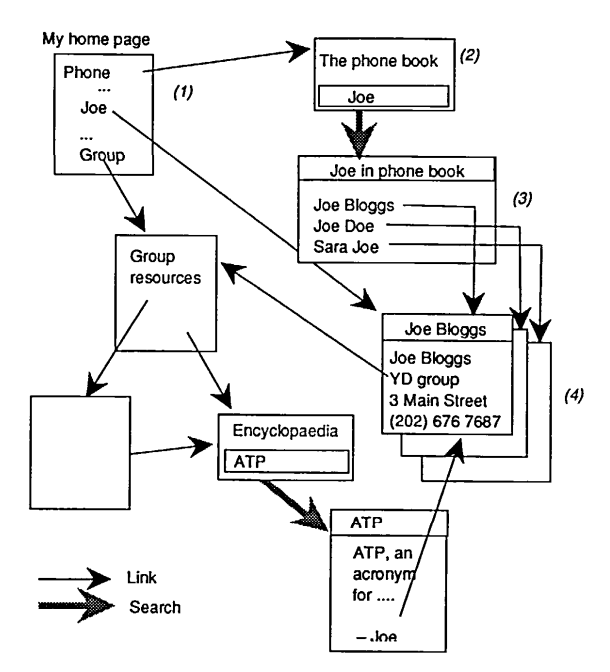
\includegraphics[keepaspectratio, width=7cm]{gambar/w3_model}
	\caption{Gambar sebuah web yang terdiri atas kumpulan \textit{link} dan indeks \citep{bernersLee1992}}
	\label{gambar:w3_model}
\end{figure}

WWW merupakan proyek Tim Berner-lee bersama teman-temannya, yang ditunjukan pada publik pada tahun 1991. WWW didesain untuk membawa sebuah semesta informasi global menggunakan teknologi yang ada. Dengan adanya WWW manusia dapat mengakses seluruh informasi melalui sebuah \textit{platform browsing} apapun. Pada masa itu, sudah ada teknologi serupa yang membuat WWW mungkin untuk dilakukan. Sistem \textit{hypertext} yang sudah ada pada saat itu, terbatas pada sistem \textit{file} lokal atau terdistribusi dan kadang hanya dikembangkan pada \textit{platform} tertentu. Selain itu, juga ada sistem pengambilan dan akses informasi seperti Alex, Gopher, Prospero, dan WAIS yang sudah mencakup area yang luas, tetapi tanpa fungsionalitas \textit{hypertext}. WWW menggabungkan teknik \textit{hypertext}, \textit{information retrieval}, dan \textit{wide area networking} \citep{bernersLee1992}.

Model yang dipakai WWW menggunakan dua paradigma dari \textit{hypertext link} dan pencarian teks yang saling melengkapi. Gambar \ref{gambar:w3_model} menunjukkan bagaimana sebuah web yang berisi informasi pribadi terbentuk pada paradigma ini. Pembaca mulai pada halaman \textit{home} (1) lalu menggunakan \textit{link} grup atau publik untuk mencari bahan informasi. Indeks seperti buku telepon (2) ditampilkan sebagai dokumen yang memungkinkan untuk melakukan input pencarian. Hasil dari pencarian berupa dokumen \textit{hypertext} virtual (3) yang menunjuk pada dokumen yang ditemukan (4) \citep{bernersLee1992}.

Terdapat fitur-fitur yang ditawarkan pada WWW yaitu:

\begin{itemize}
  \item Informasi hanya direpresentasikan sekali, sebuah rujukan (\textit{reference}) dibuat menggantikan salinan informasi.
  \item \textit{Link} memungkinkan untuk topologi informasi terus berkembang, sehingga dapat memodelkan pengetahuan manusia setiap saat tanpa kendala.
  \item Web berisi hal yang beragam mulai dari catatan kecil pada sebuah ruang kerja sampai pada basis data raksasa di benua lain.
  \item Indeks berasal dari dokumen dan dapat dicari atau melalui penelusuran \textit{link}. Sebuah indeks ditampilkan ke pengguna sebagai "halaman sampul" yang mendeskripsikan data yang diindeks dan properti dari \textit{search engine}.
  \item Dokumen pada web tidak harus memiliki bentuk fisik layaknya \textit{file}. Dokumen bisa berbentuk virtual yang dibentuk oleh server sebagai respon dari sebuah pencarian atau nama dokumen. Akibatnya dokumen dapat berbentuk \textit{views} dari basis data, atau \textit{snapshot} perubahan data.
\end{itemize}

Kebanyakan pengembangan tentang sistem \textit{hypertext} pada saat itu kebanyakan hanya berfokus pada \textit{User Interface} (UI) dan penulisan pertanyaan alih-alih pengembangan sistem yang bersifat luas (\textit{wide-area}) dan distribusi informasi dalam jangka panjang. Akibatnya, arsitektur pada sistem tersebut mengasumsikan bahwa pengguna menggunakan program aplikasi komputer yang sama pada sistem \textit{file} yang sama. Berbeda dengan WWW yang bersifat global, sehingga dihadapi dengan komputer pengguna terdistribusi dan beragam dengan tipe perangkat yang berbeda-beda. Hal ini membuat arsitektur WWW mengadopsi model klien-server. Klien bertugas memproses sebuah alamat dokumen menjadi sebuah dokumen dengan protokol jaringan tertentu. Sedangkan server menyediakan data dalam bentuk \textit{hypertext} sederhana atau dalam bentuk teks biasa, atau format data lain dengan bernegosiasi dengan klien \citep{bernersLee1992}.

Tantangan dari arsitektur tersebut adalah harus mengembangkan sebuah \textit{hypertext browser}, lebih sulit daripada mengembangkan tampilan \textit{front-end} pada sistem informasi tertentu. Walaupun demikian, memisahkan program klien dan server dengan "\textit{information bus}" akan terbayar ketika semakin banyak klien dan server bermunculan dan pembacaan universal tercapai. Menulis kode untuk sebuah server untuk data secara umum lebih sederhana karena tidak membutuhkan UI \citep{bernersLee1992}. 

\begin{figure}[H]
	\centering
	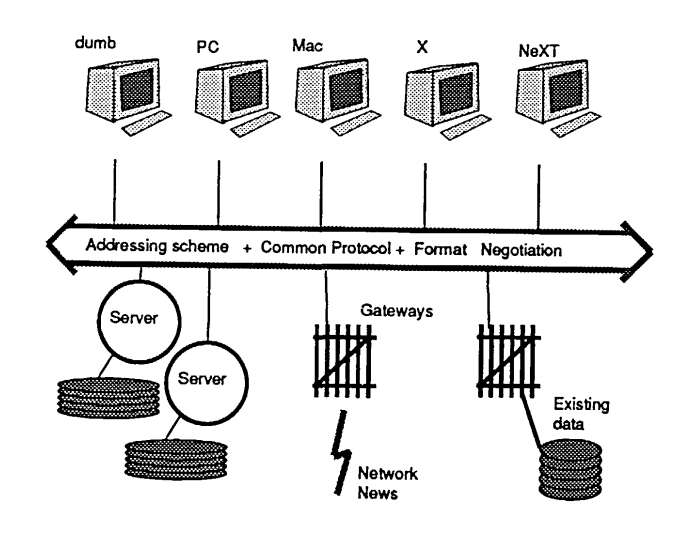
\includegraphics[keepaspectratio, width=7cm]{gambar/w3_architecture}
	\caption{Gambar arsitektur WWW \textit{link} dan indeks \citep{bernersLee1992}}
	\label{gambar:w3_architecture}
\end{figure}

Terdapat beberapa protokol yang dipakai WWW, \textit{File Transfer Protocol} (FTP), \textit{Network New Transfer Protocol} (NNTP), akses ke sistem \textit{file} terpasang (\textit{mounted}). Sebuah protokol baru yang bersifat cari dan dapatkan (\textit{search and retrieve} yang disebut HTTP, juga dianggap penting dan digunakan WWW. Lebih cepat dari FTP untuk menarik dokumen, HTTP juga memungkinkan untuk pencarian indeks. HTTP mirip dengan implementasi protokol internet yang disebutkan sebelumnya dan mirip dengan fungsionalitas protokol WAIS.

Saat ini WWW terbukti sukses dalam mewujudkan cita-citanya dalam memudahkan akses informasi global ke pengguna. Terdapat lebih dari 1 miliar situs web yang terindeks WWW \citep{huss2022} dan angka tersebut akan terus bertambah. Selain itu juga, terdapat miliaran pengguna internet yang secara otomatis juga merasakan manfaat WWW ketika melakukan pencarian di \textit{browser}. Belum lagi menyebutkan teknologi turunan yang muncul karena WWW, seperti \textit{web development}, \textit{search engine}, \textit{web API}, dan masih banyak lagi.

\section{\textit{Search Engine}}

\textit{Search engine} adalah program perangkat lunak yang memungkinkan untuk mencari kumpulan situs web berdasarkan kata kunci yang dimasukkan oleh pengguna. \textit{Search engine} lalu mencocokkan kata pencarian dengan basis data yang dimiliki. \textit{Search engine} adalah contoh sistem pengambilan informasi berskala masif \citep{seymour2011}.

Sejarah dimulai pengembangan \textit{search engine} dimulai pada tahun 1990. Alat pertama yang digunakan untuk mencari di internet adalah Archie. Archie dibuat pada 1990 oleh Alan Emtage, seorang mahasiswa di universitas McGill di Montreal. Basis data Archie terdiri atas direktori \textit{file} dari ratusan sistem. Ketika pengguna mencari di basis data Archie dalam bentuk nama \textit{file}, Archie dapat memberi tahu lokasi dari salinan \textit{file} tersebut. Archie tidak mengindeks konten dari \textit{file} tersebut. Pada periode tertentu, Archie mengunjungi situs - situs FTP terbuka yang diketahui, membuat daftar \textit{file} tersebut, dan membuat indeks yang dapat dicari. Perintah-perintah yang digunakan untuk Archie adalah perintah UNIX, sehingga untuk bisa menggunakan Archie, pengguna harus memiliki pengetahuan tentang UNIX \citep{seymour2011}.

Pada tahun 1994, seorang mahasiswa \textit{Computer Science Engineer} Universitas Washington, membuat WebCrawler pada waktu senggangnya. Awalnya WebCrawler merupakan aplikasi Desktop, bukan layanan web seperti saat ini. WebCrawler hidup di atas web dengan basis data berisi halaman dari 4000 situs web berbeda. WebCrawler merupakan \textit{search engine} web pertama yang menyediakan fitur pencarian teks secara penuh. WebCrawler berhasil dibuat pada 20 April 1994 oleh Brian Pinkerton dan dibeli America Online pada 1 Juni 1995, lalu dijual lagi ke Excite pada 1 April 1997. Yang membedakan WebCrawler dengan pendahulunya adalah penggunaan robot web pertama yang mampu mengindeks setiap kata pada halaman web, menyimpan URL, dan sebuah judul maksimal 100 kata \citep{seymour2011}.

AltaVista, dibuat pada tahun 1995, pernah menjadi \textit{search engine} yang paling populer sebelum naiknya Google. \textit{Crawler} yang dipakai AltaVista dibuat oleh Louis Moner, dan yang membuat pengindeks adalah Michael Burrows. AltaVista merupakan \textit{search engine} tercepat pada masanya yang dapat menangani jutaan \textit{hit} tiap harinya tanpa adanya penurunan performa. Satu hal yang sangat membedakan AltaVista dengan \textit{search engine} lain pada masa itu adalah mampu memproses bahasa natural sebagai kata masukan untuk mencari web. Pengguna dapat menulis kalimat atau pertanyaan untuk mendapatkan respon pintar. Sebagai contoh, pengguna dapat menulis “Dimana London ?” tanpa mendapatkan jutaan hasil pencarian yang tidak diinginkan karena mengandung “di” atau “mana” \citep{seymour2011}.

\begin{figure}[H]
	\centering
	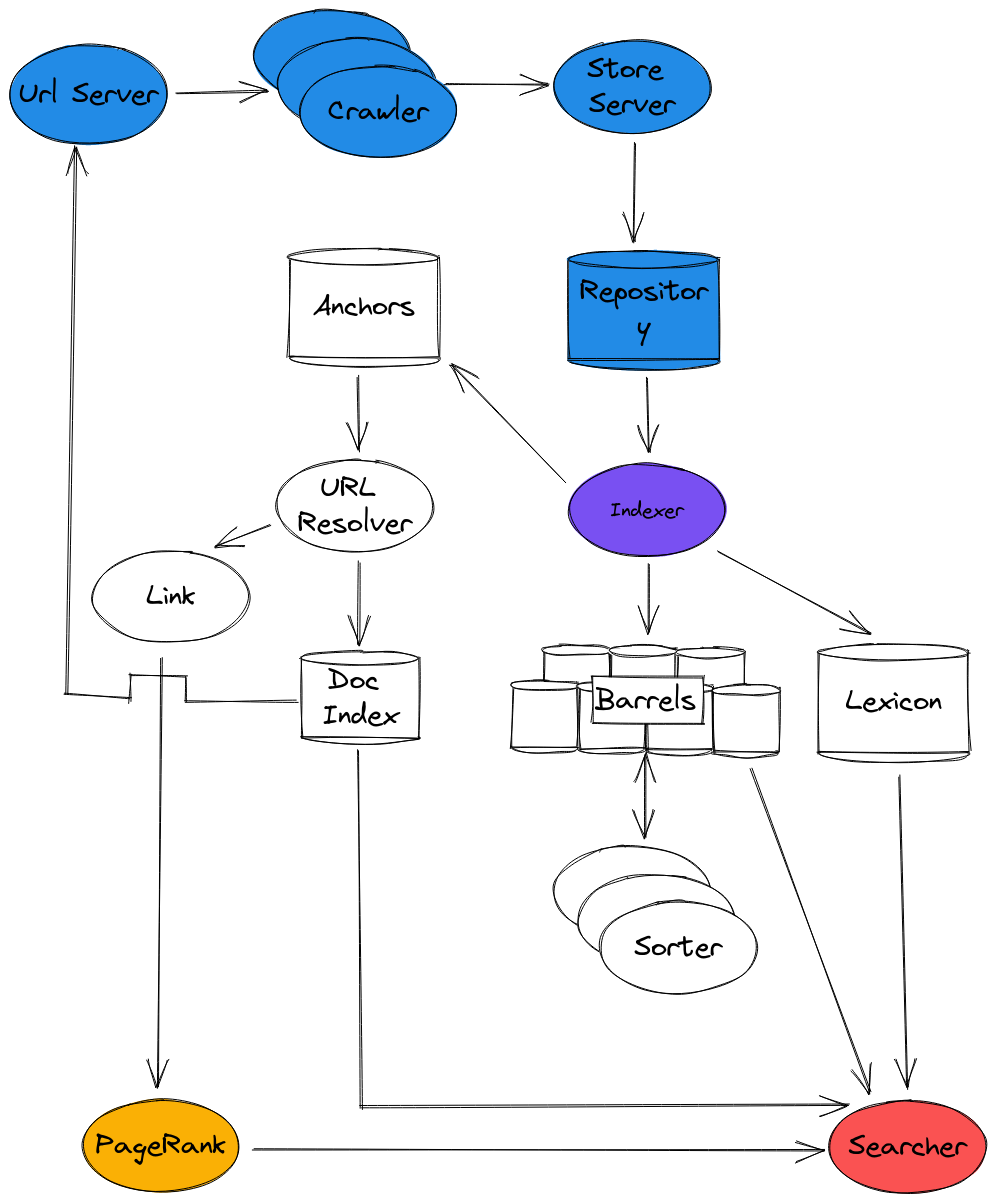
\includegraphics[keepaspectratio, width=\textwidth]{gambar/google_architecture_filled}
	\caption{\emph{High Level Google Architecture} \citep{brin1998anatomy}}
	\label{gambar:google_architecture_filled}
\end{figure}

Google dibuat pada tahun 1998, oleh Lawrence Page dan Sergey Brin. Pada saat itu, metode utama untuk menelusuri WWW adalah dengan menggunakan \textit{search engine} atau melalui situs kumpulan indeks berkualitas tinggi yang disusun oleh manusia, yang pada saat itu, yang paling populer adalah Yahoo!. Kedua metode tersebut memiliki permasalahan. Yahoo! walaupun mampu menyajikan topik - topik populer tetapi bersifat sangat subjektif, memiliki biaya yang mahal karena membutuhkan tenaga manusia, dan tidak bisa mencakup topik-topik yang bersifat esoterik \citep{brin1998anatomy}. Sedangkan untuk \textit{search engine} otomatis yang berlandaskan pada pencocokkan kata kunci biasanya menampilkan halaman web berkualitas rendah. Untuk memperburuk keadaan, pengiklan berusaha menarik perhatian pengguna dengan memanfaatkan kelemahan \textit{search engine}. Google dibuat dengan harapan untuk menjawab masalah - masalah tersebut.

Google diharapkan dapat menjadi \textit{search engine} yang \textit{scalable}, karena halaman web yang terus bertumbuh pesat. Dibutuhkan teknologi \textit{crawling} yang cepat untuk bisa mengumpulkan dokumen web dan memperbaharuinya. Perangkat penyimpanan harus digunakan seefisien mungkin untuk menyimpan indeks, dan jika memungkinkan, menyimpan dokumen web itu sendiri. Sistem pengindeksan harus bisa memproses ratusan \textit{Giga Byte} data secara efisien. Pemrosesan kueri harus ditangani secepat mungkin pada tingkat ratusan atau ribuan kueri per-detik. Hal ini juga didukung dengan semakin cepat, besar, dan murahnya perangkat keras komputer dari waktu ke waktu.

Selain \textit{scalable}, Google juga diharapkan menghasilkan hasil pencarian yang lebih berkualitas. Pada saat Google dikembangkan, hasil pencarian \textit{search engine} dipenuhi dengan hasil "sampah" karena hanya mengandalkan indeks tanpa menilai apakah halaman web yang ditampilkan memenuhi keinginan pengguna. Pengguna tidak dapat mengecek satu-per-satu dari ratusan sampai ribuan hasil pencarian yang ditampilkan. Algoritma Pagerank dikembangkan untuk Google digunakan untuk merangking seberapa penting halaman web berdasarkan struktur \textit{link} graf WWW.

Sampai saat ini, \textit{search engine} baru terus bermunculan. Pada 2004, Yahoo! yang sebelumnya terkenal sebagai direktori web, alih-alih sebagai \textit{search engine} otomatis, meluncurkan \textit{search engine} sendiri dengan menggabungkan fitur-fitur beberapa \textit{search engine} yang mereka akuisisi. Dilanjutkan pada tahun 2005 MSN Search, dan pada tahun 2009 Bing oleh Microsoft \citep{seymour2011}. Walaupun demikian, Google tetap mendominasi pasar \textit{search engine} hingga saat ini (lihat gambar \ref{gambar:search_engine_market_share}).

\begin{figure}[H]
	\centering
	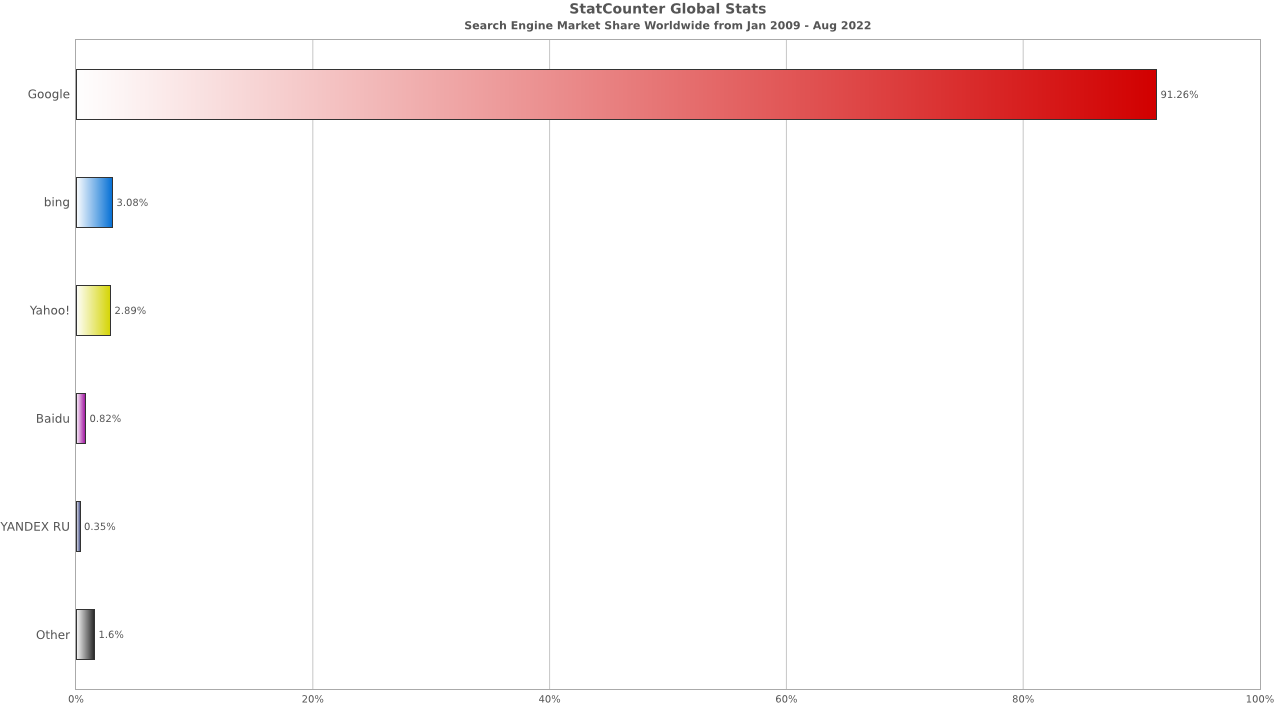
\includegraphics[keepaspectratio, width=14cm]{gambar/search_engine_market_share}
	\caption{Pangsa pasar \textit{search engine} \citep{gsc2022marketshare}}
	\label{gambar:search_engine_market_share}
\end{figure}

\section{Teori Graf}

\begin{figure}[!htb]
\begin{minipage}{0.48\textwidth}
	\centering
	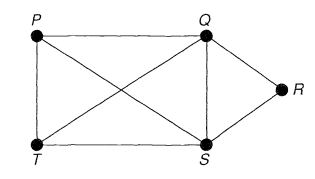
\includegraphics[width=.7\linewidth]{gambar/graph_example}
	\caption{Contoh graf \citep{wilson1996}}
	\label{gambar:graph_example}
\end{minipage}\hfill
\begin{minipage}{0.48\textwidth}
	\centering
	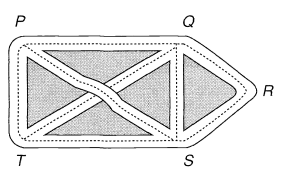
\includegraphics[width=.7\linewidth]{gambar/graph_example_2}
	\caption{Contoh peta jalan yang dapat diandaikan sebagai graf \citep{wilson1996}}
	\label{gambar:graph_example_2}
\end{minipage}
\end{figure}

\begin{figure}[H]
	\centering
	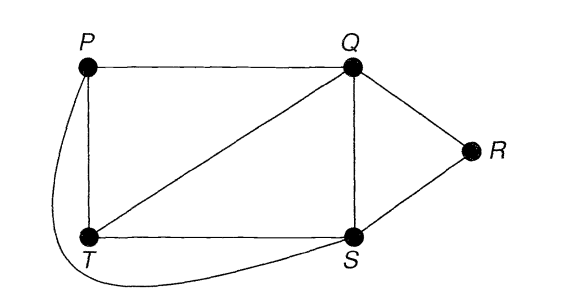
\includegraphics[keepaspectratio, width=0.48\textwidth]{gambar/graph_example_3}
	\caption{}
	\label{gambar:graph_example_3}
\end{figure}

Graf adalah sebuah representasi dari himpunan titik (\textit{node / vertice}) dan bagaimana titik-titik tersebut saling terhubung tanpa memperdulikan sifat metriknya \citep{wilson1996}. Pada gambar \ref{gambar:graph_example} merupakan contoh graf, dengan $P$, $Q$, $R$, $S$, $T$ merupakan titik, dan masing-masing terhubung dengan garis (\textit{edge}). Garis yang menghubungkan titik $P$ dan $S$ disebut dengan $PS$, sedangkan garis yang menghubungkan titik $Q$ dan $T$ disebut dengan $QT$. Persilangan antara $PS$ dan $QT$ tidak disebut sebagai titik, karena keduanya tidak saling bersilangan, melainkan saling melompati layaknya gambar \ref{gambar:graph_example_2}. Selanjutnya, kedua graf dianggap sama, jika dan hanya jika titik yang berkorespondensi sama-sama terhubung dengan garis yang sama dengan garis pada graf lainnya \citep{wilson1996}. Sebagai contoh, graf pada gambar \ref{gambar:graph_example_3} merupakan graf yang sama dengan graf pada gambar \ref{gambar:graph_example} \citep{wilson1996}. 


\begin{figure}[!htb]
\begin{minipage}{0.48\textwidth}
	\centering
	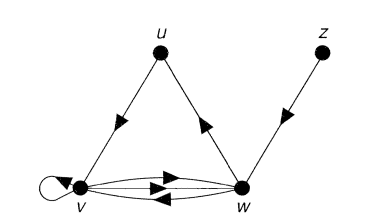
\includegraphics[width=.7\linewidth]{gambar/digraph_example}
	\caption{Contoh digraf \citep{wilson1996}}
	\label{gambar:digraph_example}
\end{minipage}\hfill
\begin{minipage}{0.48\textwidth}
	\centering
	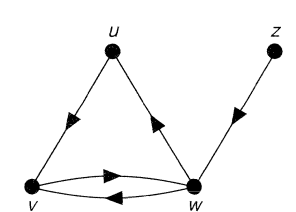
\includegraphics[width=.7\linewidth]{gambar/simple_digraph_example}
	\caption{Contoh digraf sederhana \citep{wilson1996}}
	\label{gambar:simple_digraph_example}
\end{minipage}
\end{figure}

Garis pada graf dapat diberikan arah. Garis pada graf yang berarah disebut sebagai busur (\textit{arc}). Graf yang memiliki arah pada garisnya disebut dengan graf berarah (\textit{directed graph / digraph} / digraf) yang terdiri atas himpunan titik dan busur \citep{wilson1996}. Pada digraf di gambar \ref{gambar:digraph_example} terdapat himpunan titik $u$, $v$, $w$, dan $z$, dengan busur $uv$, $vv$, $vw (2\times)$, $wv$, $wu$, dan $zw$. Sebuah digraf disebut sebagai digraf sederhana jika himpunan busurnya tidak ada yang sama (\textit{distinct}) dan tidak memiliki \textit{loop} (contoh: busur $vv$) \citep{wilson1996}. Digraf pada gambar \ref{gambar:simple_digraph_example} adalah contoh digraf sederhana.

\section{Pagerank}

World Wide Web memberikan tantangan baru dalam hal memperoleh informasi karena besar dan beragam isi-nya. Terdapat miliaran halaman web saat ini. Halaman web tersebut sangat beragam mulai dari "Apa yang Joe makan hari ini ?" sampai ke jurnal tentang \textit{information retrieval}. Belum lagi tantangan lain \textit{search engine} harus menghadapi pengguna yang kurang berpengalaman dan banyaknya halaman web yang sudah dibuat sedemikian rupa untuk memanipulasi fungsi perangkingan yang dipakai \textit{search engine}.

Walaupun demikian, tidak seperti dokumen biasa, halaman web berisi \textit{hypertext} dan menyediakan banyak informasi tambahan pada setiap teks yang ada pada halaman web, seperti struktur \textit{link} dan \textit{link} teks. Pagerank memanfaatkan keuntungan struktur \textit{link} pada web untuk menghasilkan sebuah \textit{ranking} seberapa penting pada setiap halaman web secara global. \textit{Ranking} ini membantu \textit{search engine} dan pengguna untuk menelusuri luas dan beragamnya World Wide Web.

Jika World Wide Web diibaratkan pada sebuah graf berarah, halaman web adalah titik graf, \textit{link} adalah garis. Lalu \textit{link} yang menunjuk keluar dari titik disebut \textit{forward link}, sedangkan \textit{link} yang menunjuk kedalam titik disebut \textit{backlink} (Lihat gambar \ref{gambar:web_graph_ilustration}). Sangat sulit untuk mengetahui semua \textit{backlink} suatu halaman web, tetapi sangat mudah untuk mengetahui semua \textit{forward link} suatu halaman web yaitu dengan cara mengunduh halaman web tersebut \citep{ilprints422}. Setiap halaman web memiliki jumlah \textit{backlink} yang beragam. Pada saat Pagerank diteliti, halaman \textit{home} NetScape memiliki 62.804 \textit{backlink} dibandingkan halaman web kebanyakan yang hanya memiliki beberapa \textit{backlink}. Secara umum suatu halaman web jika memiliki banyak \textit{backlink} dapat dianggap lebih penting daripada halaman web lain yang memiliki lebih sedikit \textit{backlink}. Perhitungan jumlah sitasi sederhana pernah digunakan untuk memprediksi pemenang Nobel masa depan \citep{ilprints422}. 

\begin{figure}[H]
	\centering
	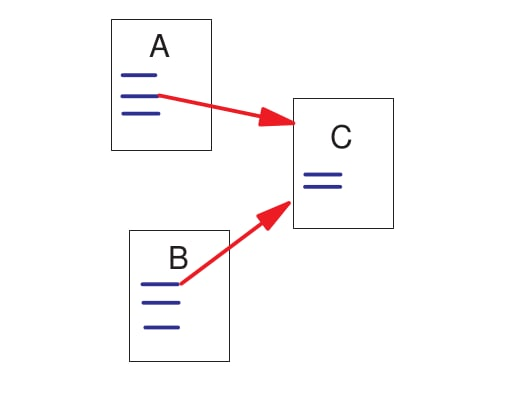
\includegraphics[keepaspectratio, width=7cm]{gambar/web_graph_ilustration}
	\caption{A dan B adalah \textit{backlink} dari C \citep{ilprints422}}
	\label{gambar:web_graph_ilustration}
\end{figure}

Yang membuat Pagerank menarik adalah sekedar menghitung jumlah sitasi atau \textit{backlink} saja tidak cukup untuk membuat \textit{ranking} halaman web sesuai dengan apa yang pengguna anggap sebagai penting. Sebagai contoh, jika ada suatu halaman web yang memiliki \textit{backlink} dari situs terkenal, misal halaman \textit{home} Yahoo.com, mungkin itu hanya satu \textit{link} tetapi berasal dari halaman yang penting. Halaman tersebut seharusnya memiliki \textit{ranking} di atas halaman web yang memiliki banyak \textit{backlink} tetapi berasal dari tempat yang tidak jelas. Pagerank berusaha untuk mewujudkan perangkingan yang selaras dengan makna penting di mata pengguna hanya dengan menggunakan struktur \textit{link} \citep{ilprints422}.

Pagerank dapat didefinisikan pada persamaan \ref{eq:1}. Halaman web merupakan $u$. Himpunan $F_u$ adalah kumpulan halaman $u$ yang menunjuk halaman lain atau disebut dengan \textit{forward link} dan $B_u$ adalah himpunan halaman yang menunjuk ke $u$ atau disebut dengan \textit{backlink}. $C_u = |F_u|$ adalah jumlah \textit{link} dari $u$, sedangkan $c$ adalah faktor yang digunakan untuk normalisasi (sehingga jumlah total \textit{ranking} semua halaman web adalah konstan) dan $c < 1$. $E(u)$ adalah vektor yang berkorespondensi dengan \textit{ranking} halaman web. $||\pi'||_1 = 1$. Iterasi perhitungan terus dilakukan sampai konvergen. Jika diubah kedalam persamaan matriks, maka persamaan \ref{eq:1} dapat diubah menjadi persamaan \ref{eq:2}. Dimana $X$ adalah matriks persegi yang baris dan kolomnya berkorespondensi dengan halaman web, dengan elemen $X_{u,v} = \frac{1}{C_v}$ jika terdapat \textit{link} pada halaman $v$ ke halaman $u$ atau $X_{u,v} = 0$ jika tidak ada.

Berdasarkan persamaan \ref{eq:2}, Algoritma Pagerank secara sederhana dapat didefinisikan pada algoritma \ref{alg:1}. Vektor ranking awal-awal dapat didefinisikan sebagai vektor apapun yang berkorespondensi dengan halaman web (misal $E$). 

\begin{breakablealgorithm}
\label{alg:1}
\floatname{algorithm}{Algoritma}
\caption{Algoritma Pagerank \citep{ilprints422}}
\begin{algorithmic}[1]
  \State $\pi_0 \gets \text{vektor ranking awal-awal (misal $E$)}$
  \Do
    \State $\pi_{i+1} \gets X\pi_i$
    \State $\delta \gets ||\pi_i||_1 - ||\pi_{i+1}||_1$
    \State $\pi_{i+1} \gets \pi_{i+1} + \delta E$
  \doWhile{$||\pi_{i+1} - \pi_i||_1 > \epsilon$}
\end{algorithmic}
\end{breakablealgorithm}

\section{\textit{Distributed Pagerank Computation} (DPC)}

Telah dijelaskan sebelumnya, masalah dari algoritma Pagerank biasa adalah besarnya memori utama yang dibutuhkan untuk bisa menyimpan matriks $X$ (lihat persamaan \ref{eq:2}). Oleh karena itu, dirumuskan algoritma Pagerank terdistribusi. DPC, dirumuskan oleh \citet{zhuetal2005distributedPagerank}, memakai mekanisme interaksi sederhana antara \textit{cluster} dan lalu lintas komunikasi rendah. Ditinjau dari perspektif matematika, dibuktikan bahwa algoritma DPC setara dengan metode \textit{Iterative Aggregation-Disaggregation} (IAD) dengan \textit{Block Jacobi smoothing}. DPC juga memiliki keunggulan dibandingkan dengan algoritma Pagerank biasa yaitu, matriks-matriks dipecah menjadi matriks agregasi dan matriks lokal sehingga ukurannya cukup kecil untuk disimpan di memori utama, sehingga mempercepat komputasi karena tiap iterasi memerlukan sedikit operasi I/O pada \textit{disk}. Selanjutnya, Vektor Pagerank lokal konvergen lebih cepat pada beberapa \textit{cluster} tertentu, berbeda dengan Pagerank biasa karena terdapat komputasi tidak perlu pada \textit{cluster} yang sudah konvergen \citep{zhuetal2005distributedPagerank}.

\subsection{Algoritma Pagerank versi DPC}

Secara esensi algoritma Pagerank pada artikel asli \citet{ilprints422}, dan algoritma Pagerank yang dipakai pada algoritma DPC pada artikel \citet{zhuetal2005distributedPagerank} adalah sama. Hanya terdapat beberapa penyesuaian. Pertama vektor $E$, merupakan probabilitas \textit{random walker} melompat ke halaman web lain secara acak, diganti dengan $(1 - d)$. $d$ disebut sebagai \textit{damping factor} merupakan probabilitas \textit{random walker} mengikuti \textit{link} yang tersedia. Nilai $d$ pada penelitian \citet{zhuetal2005distributedPagerank} adalah $0.85$. Yang kedua, jika vektor $E$ pada algoritma Pagerank di artikel \citet{ilprints422} digunakan pada langkah tersendiri, sedangkan nilai $d$ pada artikel \citet{zhuetal2005distributedPagerank} dipakai langsung dalam menentukan nilai elemen pada matriks transisi.

\begin{equation}
	\label{eq:5-1}
	P_{ij}= 
	\begin{cases}
		\frac{d}{C_j} + \frac{(1-d)}{N} & j \to i \\
		\frac{(1-d)}{N} & j \not\to i \text{ dan } C_j \not=0 \\
		\frac{1}{N} & C_j = 0
	\end{cases}
\end{equation}

Matriks transisi pada algoritma DPC didefinisikan sebagai matriks $P$. Matriks $P$ didefinisikan pada persamaan \ref{eq:5-1}. $C_j$ adalah jumlah \textit{forward link} dari halaman $j$. $j \to i$ adalah halaman $j$ memiliki \textit{link} menuju halaman $i$.

Selanjutnya algoritma Pagerank yang dipakai DPC didefinisikan pada algoritma \ref{alg:1.1}

\begin{breakablealgorithm}
	\label{alg:1.1}
	\floatname{algorithm}{Algoritma}
	\caption{Algoritma Pagerank yang dipakai DPC \citep{zhuetal2005distributedPagerank}}
	\begin{algorithmic}[1]
		\State Definisikan $\pi^0$ awal-awal
		\State $k \gets 0$
		\State \label{alg:1.1.step:start_loop} $\pi^{\sim k+1} \gets P \pi^k$
		\State $\pi^{k+1} \gets \frac{\pi^{\sim k+1}}{||\pi^{\sim k+1}||_1}$
		\State Jika $||\pi^{k+1} - \pi^k|| < \epsilon$  berhenti dan kembalikan nilai $\pi^{k+1}$
		\State $k \gets k+1$
		\State Ulangi langkah \ref{alg:1.1.step:start_loop}
	\end{algorithmic}
\end{breakablealgorithm}

\subsection{Algoritma IAD}

Jika \textit{link} pada kumpulan web dibuat kedalam graf, maka graf tersebut akan memiliki sebuah struktur menyerupai blok, karena mayoritas dari \textit{link} tersebut bersifat \textit{intra-host}, merujuk halaman yang masih di dalam \textit{host} yang sama. Oleh karena itu, jika dilakukan perjalanan acak pada kumpulan web tersebut dapat dilihat sebagai rantai Markov \textit{Nearly Completely Decomposable} (NCD) \citep{zhuetal2005distributedPagerank}. Rantai Markov NCD adalah rantai Markov yang dapat dipartisi sehingga peluang dari keadaan awal ke keadaan selanjutnya lebih sering menunjuk keadaan yang berada di dalam partisinya dibandingkan di luar partisinya \citep{kontovasilisMitrou1995}. Sebelum dijelaskan tentang DPC, akan dijelaskan metode IAD terlebih dahulu.

Misal G adalah himpunan bilangan bulat $\{1,...,N\}$. Misal $G_1,...G_n, n \leq N$ adalah grup agregasi dari elemen-elemen di $G$. Himpunan-himpunan $G_i, i = 1,...,n$, adalah saling lepas dan $\cup^n_{i=1}G_i=G$. Misal $N_i$ adalah ordo dari himpunan $G_i$, atau jumlah elemen-elemen di $G_i$ \citep{zhuetal2005distributedPagerank}. 

Misal $R$ adalah matriks agregasi $n \times N$, yang memenuhi persamaan \ref{eq:3} \citep{zhuetal2005distributedPagerank}.

\begin{equation}
	\label{eq:3}
	R_{ij}= 
	\begin{cases}
			1 & j \in G_i\\
			0 & \text{lainnya}
	\end{cases}
\end{equation}

Dilakukan partisi pada vektor positif $\pi$ menjadi $(\pi^T_1,\pi^T_2,...,\pi^T_n)^T$ berdasarkan $\{G_i\}$. $\pi_i$ adalah subvektor dengan dimensi $N_i$ \citep{zhuetal2005distributedPagerank}.

Maka dapat didefinisikan matriks disagregasi $S(\pi)$ $N \times n$ sebagai persamaan \ref{eq:4} \citep{zhuetal2005distributedPagerank}.
\begin{equation}
	\label{eq:4}
	S(\pi) = 
	\begin{pmatrix}
		S(\pi)_1 & 0 & \ldots & 0 \\
		0 & S(\pi)_2 & \ldots & 0 \\
		\vdots & \vdots & \ddots & \vdots \\
		0 & 0 & \ldots & S(\pi)_n
	\end{pmatrix}
\end{equation}
Dimana $S(\pi)_i$ adalah sebuah kolom vektor yang mewakili \textit{censored stationary distribution} dari halaman-halaman di \textit{cluster} $G_i$. Ingat bahwa $RS(\pi) = I$ \citep{zhuetal2005distributedPagerank}.

\begin{breakablealgorithm}
	\label{alg:2}
	\floatname{algorithm}{Algoritma}
	\caption{Algoritma IAD \citep{zhuetal2005distributedPagerank}}
	\begin{algorithmic}[1]
		\State $||\pi^0|| \gets 1$
		\State $\pi^0 \gets$ Pilih bilangan bulat positif
		\State $k \gets 0$
		\Do
			\State Buat matriks agregasi $RPS(\pi^k)$ dan selesaikan persamaan linear \ref{eq:5}. Dimana $||z|| = 1$
			\begin{equation}
				\label{eq:5}
				RPS(\pi^k)z^k = z^k
			\end{equation}
			\State $\pi^{\sim k+1} \gets TS(\pi^k)z^k$
			\State $\pi^{k+1} \gets \frac{\pi^{\sim k+1}}{||\pi^{\sim k+1}||_1}$
			\State $k \gets k + 1$
		\doWhile{$||\pi^{k+1} - \pi^k|| < \epsilon$}
	\end{algorithmic}
\end{breakablealgorithm}

Misal $T = M^{-1}N$ adalah sebuah matriks berasal dari operasi pemisahan matriks dari $I - P = M - N$. Dimana $M$ adalah matriks non-singular (bisa dilakukan invers) dan operasi pemisahan matriksnya adalah \textit{weak regular}, yang berarti $M^{-1} \geq 0$ dan $M^{-1}N \geq 0$ \citep{mishra2016}. Untuk menyelesaikan persamaan linear $(I - P)\pi = 0$, maka dapat dirumuskan algoritma Iteration Aggregation Disaggregation (IAD) yang dapat dilihat pada algoritma \ref{alg:2} \citep{zhuetal2005distributedPagerank}.

\subsection{Algoritma DPC}

Sebelum langsung membahas algoritma DPC, akan didefinisikan beberapa notasi terlebih dahulu. $e=(1,...,1)^T$. Matriks transisi $P$ dipartisi menjadi beberapa blok berdasarkan $\{G_i\}$ menjadi seperti persamaan \ref{eq:6} \citep{zhuetal2005distributedPagerank}.
\begin{equation}
\label{eq:6}
	P =
	\begin{pmatrix}
		P_{11} & P_{12} & \ldots & P_{1n} \\
		P_{21} & P_{22} & \ldots & P_{2n} \\
		\vdots & \vdots & \ddots & \vdots \\
		P_{n1} & P_{n2} & \ldots & P_{nn}
	\end{pmatrix}
\end{equation}
Dilambangkan blok baris ke-$i$ sebagai persamaan \ref{eq:7}
\begin{equation}
\label{eq:7}
	P_{i*} \overset{\Delta}{=} (P_{i1},\ldots,P_{in})
\end{equation}
dan dilambangkan blok kolom ke-$i$ sebagai persamaan \ref{eq:8}
\begin{equation}
\label{eq:8}
	P_{*i} \overset{\Delta}{=}
	\begin{pmatrix}
		P_{1i} \\
		\vdots \\
		P_{ni} 
	\end{pmatrix}
\end{equation} 

Setiap blok diagonal $P_{ii}$ adalah matriks persegi dan merupakan matriks \textit{intra-cluster} \textit{link} dari \textit{cluster} $G_i$, sementara blok-blok di luar diagonal merupakan struktur \textit{link} antar-\textit{cluster}. Selanjutnya, matriks agregat $A = RPS(\pi)$ adalah matriks transisi antar \textit{cluster}. Maka dapat dibuat algoritma DPC pada algoritma \ref{alg:3} \citep{zhuetal2005distributedPagerank}.

\begin{breakablealgorithm}
\label{alg:3}
\floatname{algorithm}{Algoritma}
\caption{Algoritma DPC \citep{zhuetal2005distributedPagerank}}
\begin{algorithmic}[1]
  \State Buat matriks transisi lokal untuk tiap \textit{cluster} $G_i$ berdasarkan $P$ 
		\begin{equation} \label{alg:3.step:trivial:1} Q_i = LocalTransitionMatrix(G_i) \forall G_i \in G \end{equation}
  \State 
		\begin{equation} \label{alg:3.step:trivial:2} \pi_i^0 = Pagerank(Q_i, \frac{e}{N_i}, \epsilon) \forall G_i \in G \end{equation}
		Ket: $e = [1, 1, ..., 1]^T; N_i \rightarrow \text{jumlah anggota $G_i$}$
  \State Inisialisasi $k = 0$
	\State
		\begin{equation} \label{alg:3.step:2:1} A^k = RPS(\pi^k) \end{equation}
		Ket: $R \rightarrow \text{persamaan \ref{eq:3}}; P \rightarrow \text{persamaan \ref{eq:5-1}}; S(\pi) \rightarrow \text{persamaan \ref{eq:4}}$
	\State
		\begin{equation} \label{alg:3.step:2:2} z^k = Pagerank(A^k, \frac{e}{n}, \epsilon) \end{equation}
		Ket: $n \rightarrow \text{banyaknya anggota }G$
	\State \label{alg:3.step:3:1} $\forall G_i \in G$ buat sebuah \textit{extended local transition matrix} $(N_i + 1) \times (N_i + 1)$. Dimana skalar $\alpha^k$ membuat jumlah nilai kolom dari $B^k_i$ adalah satu
		\begin{equation}
			\label{eq:9}
			B_i^k =
			\begin{pmatrix}
				P_{ii} 		& \frac{(P_{i*}S(\pi^k)z^k - P_{ii}\pi_i^kz_i)}{(1 - z^k_i)} \\
				e^TP_{*i} & \alpha^k
			\end{pmatrix}
		\end{equation}
	\State \label{alg:3.step:3:2} Hitung vektor \textit{extended local Pagerank}. Dimana $\beta^{k+1}_i$ adalah skalar
		\begin{equation}
			\begin{pmatrix}
				\omega^{k+1}_i \\
				\beta^{k+1}_i
			\end{pmatrix}
			= Pagerank(B^k_i, \frac{e}{(N_i + 1)}, \epsilon)
		\end{equation}
	\State \label{alg:3.step:3:3} \begin{equation} \pi^{\sim k+1}_i = \frac{1 - z^k_i}{\beta^{k+1}_i} \omega^{k+1}_i \end{equation}
	\State \label{alg:3.step:normalization} \begin{equation} \pi^{k+1} = \frac{\pi^{\sim k+1}}{||\pi^{\sim k+1}||_1} \end{equation}
	\State $k = k+1$
	\State Jika persamaan \ref{alg:3.eq:1} terpenuhi, berhenti dan berikan $\pi^{k}$ sebagai hasil akhir. Jika sebaliknya, kembali ke langkah \ref{alg:3.step:2:1}
		\begin{equation} \label{alg:3.eq:1} ||\pi^{k+1} - \pi^k|| < \epsilon \end{equation}
\end{algorithmic}
\end{breakablealgorithm}

\subsection{Contoh Nilai dari tiap simbol algoritma DPC}

Akan diberikan contoh nilai dari tiap simbol algoritma DPC yang sudah dijelaskan sebelumnya. Misal diberikan graf berarah halaman web pada gambar \ref{gambar:web_graph}. Jika dibuat matriks $P$, berdasarkan persamaan \ref{eq:5-1}, dan jika $d = 0,85$, maka matriks P yang terbentuk akan menjadi seperti matriks \ref{eq:p_matrix_example}. Nilai dari elemen $P_{1,1}$ diperoleh dari perhitungan $\frac{1 - d}{N} = \frac{1 - 0,85}{7} = 0,02143$, karena antara halaman 1 ("unj.ac.id") tidak memiliki \textit{forward link} ke dirinya sendiri. Nilai dari elemen $P_{2,1}$ diperoleh dari perhitungan  $\frac{d}{C_j} + \frac{1 - d}{N} = \frac{0,85}{5} + \frac{1 - 0,85}{7} = 0,23393$ karena antara halaman 1 memiliki \textit{forward link} ke halaman 2 ("unj.ac.id/sejarah-unj"). Nilai elemen $P_{1,2}$ sampai elemen $P_{7,2}$ diperoleh dari perhitungan $\frac{1}{N} = \frac{1}{7} = 0,14286$, karena halaman 2 tidak memiliki \textit{forward link} ke halaman manapun.

\begin{figure}[H]
	\centering
	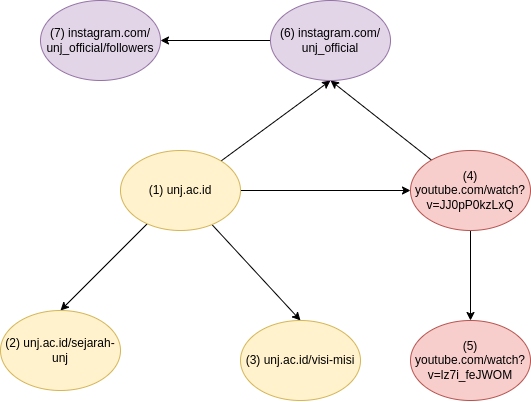
\includegraphics[height=7cm, keepaspectratio]{gambar/web_graph}
	\caption{}
	\label{gambar:web_graph}
\end{figure}

\begingroup
\makeatletter
\def\f@size{10}
\check@mathfonts
\begin{equation}
\label{eq:p_matrix_example}
	P =
	\begin{pmatrix}
		0,02143 & 0,14286 & 0,14286 & 0,02143 & 0,14286 & 0,02143 & 0,14286 \\
		0,23393 & 0,14286 & 0,14286 & 0,02143 & 0,14286 & 0,02143 & 0,14286 \\
		0,23393 & 0,14286 & 0,14286 & 0,02143 & 0,14286 & 0,02143 & 0,14286 \\
		0,23393 & 0,14286 & 0,14286 & 0,02143 & 0,14286 & 0,02143 & 0,14286 \\
		0,02143 & 0,14286 & 0,14286 & 0,44643 & 0,14286 & 0,02143 & 0,14286 \\
		0,23393 & 0,14286 & 0,14286 & 0,44642 & 0,14286 & 0,02143 & 0,14286 \\
		0,02143 & 0,14286 & 0,14286 & 0,02143 & 0,14286 & 0,87143 & 0,14286 \\
	\end{pmatrix}
\end{equation}
\endgroup

Dari matriks P sebelumnya, maka dapat dipecah layaknya pada persamaan \ref{eq:6}, menjadi matriks \ref{eq:separated_p_matrix_example}.

\begin{equation}
\label{eq:separated_p_matrix_symbol}
	P =
	\begin{pmatrix}
		P_{1,1} & P_{1,2} & P_{1,3} \\
		P_{2,1} & P_{2,2} & P_{2,3} \\
		P_{3,1} & P_{3,2} & P_{3,3} \\
	\end{pmatrix}
\end{equation}

\begingroup
\makeatletter
\def\f@size{8}
\check@mathfonts
\begin{equation}
\label{eq:separated_p_matrix_example}
	P =
	\begin{pmatrix}
		\begin{pmatrix}
			0,02143 & 0,14286 & 0,14286 \\
			0,23393 & 0,14286 & 0,14286 \\
			0,23393 & 0,14286 & 0,14286 \\
		\end{pmatrix} &
		\begin{pmatrix}
			0,02143 & 0,14286 \\
			0,02143 & 0,14286 \\
			0,02143 & 0,14286 \\
		\end{pmatrix} &
		\begin{pmatrix}
			0,02143 & 0,14286 \\
			0,02143 & 0,14286 \\
			0,02143 & 0,14286 \\
		\end{pmatrix} \\ \\

		\begin{pmatrix}
			0,23393 & 0,14286 & 0,14286 \\
			0,02143 & 0,14286 & 0,14286 \\
		\end{pmatrix} &
		\begin{pmatrix}
			0,02143 & 0,14286 \\
			0,44643 & 0,14286 \\
		\end{pmatrix} &
		\begin{pmatrix}
			0,02143 & 0,14286 \\
			0,02143 & 0,14286 \\
		\end{pmatrix} \\ \\

		\begin{pmatrix}
			0,23393 & 0,14286 & 0,14286 \\
			0,02143 & 0,14286 & 0,14286 \\
		\end{pmatrix} &
		\begin{pmatrix}
			0,44642 & 0,14286 \\
			0,02143 & 0,14286 \\
		\end{pmatrix} &
		\begin{pmatrix}
			0,02143 & 0,14286 \\
			0,87143 & 0,14286\\
		\end{pmatrix} \\
	\end{pmatrix}
\end{equation}
\endgroup

Dari matriks $P_{1,1}$, $P_{2,2}$, dan $P_{3,3}$ dapat diperoleh matriks transisi lokal $Q_1$, $Q_2$, dan $Q_3$ yang tiap kolomnya dinormalisasi yang dapat dilihat pada matriks \ref{eq:q_i_example}.

\begingroup
\makeatletter
\def\f@size{10}
\check@mathfonts
\begin{align}
\label{eq:q_i_example}
	Q_1 =
	\begin{pmatrix}
		0,0438 & 0,33333 & 0,33333 \\
		0,4781 & 0,33333 & 0,33333 \\
		0,4781 & 0,33333 & 0,33333 \\
	\end{pmatrix} &
	Q_2 =
	\begin{pmatrix}
		0,0458 & 0,5 \\
		0,9542 & 0,5 \\
	\end{pmatrix} &
	Q_3 =
	\begin{pmatrix}
		0,024 & 0,5 \\
		0,976 & 0,5 \\
	\end{pmatrix}
\end{align}
\endgroup

Selanjutnya dari graf di gambar \ref{gambar:web_graph} dapat ditemukan 3 domain, yaitu domain 1 adalah "unj.ac.id" dengan anggota halaman "unj.ac.id", "unj.ac.id/sejarah-unj", dan "unj.ac.id/visi-misi" yang dapat dinotasikan sebagai $G_1 = \{1, 2, 3\}$. Domain 2 adalah "youtube.com" dengan anggota halaman "youtube.com/watch?v=JJ0pP0kzLxQ" dan "youtube.com/watch?v=lz7i$\_$feJWOM" yang dapat dinotasikan sebagai $G_2 = \{4, 5\}$. Yang terakhir domain 3 "instagram.com" dengan anggota halaman "instagram.com/unj$\_$official" dan "instagram.com/unj$\_$official/followers" $G_3 = \{6, 7\}$. Jika dibuat matriks R maka dapat dilihat pada matriks \ref{eq:r_matrix_example}. Elemen $R_{1,1}$ sampai elemen $R_{1,3}$ mendapat nilai 1 karena halaman 1 sampai 3 merupakan anggota $G_1$, sedangkan elemen $R_{1,4}$ sampai elemen $R_{1,7}$ mendapat nilai 0 karena halaman 4 sampai 7 bukan anggota $G_1$.

\begin{equation}
\label{eq:r_matrix_example}
	R =
	\begin{pmatrix}
		1 & 1 & 1 & 0 & 0 & 0 & 0 \\
		0 & 0 & 0 & 1 & 1 & 0 & 0 \\
		0 & 0 & 0 & 0 & 0 & 1 & 1 \\
	\end{pmatrix}
\end{equation}

Pada setiap halaman web tersebut, pada tiap anggota domain-nya dapat dijalankan algoritma Pagerank. Setelah konvergen, keluaran dari algoritma Pagerank pada tiap domainnya adalah beberapa vektor $S(\pi)_1 = \{0,25974; 0,37013;  0,37013\}$, $S(\pi)_2 = \{0,35088; 0,64912\}$, dan $S(\pi)_3 = \{0,35088; 0,64912\}$. Jika dibuat matriks $S(\pi)$ maka akan terbentuk matriks \ref{eq:s_phi_matrix_example}.

\begingroup
\makeatletter
\def\f@size{10}
\check@mathfonts
\begin{equation}
\label{eq:s_phi_matrix_example}
	S(\pi) =
	\begin{pmatrix}
		0,25974 & 0 & 0 \\
		0,37013 & 0 & 0 \\
		0,37013 & 0 & 0 \\
		0 & 0,35088 & 0 \\
		0 & 0,64912 & 0 \\
		0 & 0 & 0,35088 \\
		0 & 0 & 0,64912 \\
	\end{pmatrix}
\end{equation}
\endgroup

Setelah diperoleh matriks $R$, $P$, $S(\pi)$ maka dapat diperoleh matriks $A$, dengan mengalikan ketiga matriks tersebut, sehingga memperoleh matriks \ref{eq:a_matrix_example}.

\begin{equation}
\label{eq:a_matrix_example}
	A =
	\begin{pmatrix}
		0,44434882 & 0,30075792 & 0,30075792 \\
		0,27783429 & 0,34962928 & 0,20050528 \\
		0,27783429 & 0,34962577 & 0,49875328 \\
	\end{pmatrix}
\end{equation}

Selanjutnya diperoleh vektor $z$ dengan melakukan perhitungan Pagerank sampai konvergen dengan memasukan matriks $A$ sebagai matriks transisi, dan vektor $\frac{e}{n} = [\frac{1}{3}, \frac{1}{3}, \frac{1}{3}]^T$ sebagai vektor \textit{ranking} awal-awal. Hasil dari vektor $z$ dapat dilihat pada vektor \ref{eq:z_vector_example}.      

\begin{equation}
\label{eq:z_vector_example}
	z =
	\begin{pmatrix}
		0,35118 \\ 
		0,26756 \\ 
		0,38127 \\
	\end{pmatrix}
\end{equation}

Dari vektor dan matriks sebelumnya dapat dibentuk matriks $B_i$. Karena terdapat 3 domain, maka matriks $B_i$ yang terbetuk adalah matriks $B_1$, $B_2$, dan $B_3$. Proses pembentukan matriks $B_1$ dapat dilihat pada persamaan \ref{eq:b_1_example}.

\begin{align}
\label{eq:b_1_example}
	B_1 & = & 
	\begin{pmatrix}
		P_{1,1} & \frac{P_{1,\ast} \times S(\pi) \times z - P_{1,1} \times \pi_1 \times z_1}{1 - z_1} \\
		e^T \times P_{\ast,1} & \alpha
	\end{pmatrix} \nonumber \\
	%%%%%
	& = &
	\begin{pmatrix}
		\begin{pmatrix}
			0,02143 & 0,14286 & 0,14286 \\
			0,23393 & 0,14286 & 0,14286 \\
			0,23393 & 0,14286 & 0,14286 \\
		\end{pmatrix} & 
		\begin{pmatrix}
			0,10025 \\ 
			0,10025 \\ 
			0,10025 \\
		\end{pmatrix} \\\\
		\begin{pmatrix}
			1,00001 & 1,00002 & 1,00002
		\end{pmatrix} & 
		\begin{pmatrix}
			0,69924
		\end{pmatrix}
	\end{pmatrix} \\ \nonumber
	%%%%%%%
	& = &
	\begin{pmatrix}
		0,02143 & 0,14286 & 0,14286 & 0,10025 \\
		0,23393 & 0,14286 & 0,14286 & 0,10025 \\
		0,23393 & 0,14286 & 0,14286 & 0,10025 \\
		1,00001 & 1,00002 & 1,00002 & 0,69924 \\
	\end{pmatrix} \\ \nonumber
\end{align}

Dari \textit{extended local matrix} $B_1$ dapat diperoleh \textit{local pagerank vector} untuk domain 1. Vektor yang diperoleh dapat dilihat pada vektor \ref{eq:extended_local_pagerank_vector_example}. Di mana elemen baris 1 sampai baris 3 merupakan nilai vektor $\omega_1$, sedangkan baris 4 merupakan nilai $\beta_1$.

\begin{equation}
\label{eq:extended_local_pagerank_vector_example}
	\begin{pmatrix}
		\omega_1 \\
		\beta_1
	\end{pmatrix}
	=
	\begin{pmatrix}
		0,09005 \\
		0,10689 \\
		0,10689 \\
		0,69617
	\end{pmatrix}
\end{equation}

\subsection{Analisis Konvergen}

Dibuktikan konvergensi metode \textit{Block Jacobi} pada skenario Pagerank. Pertama-tama diberikan sebuah lema yang diambil dari penelitian \citet{courtoisSemal1986} \citep{zhuetal2005distributedPagerank}:

\textbf{Lema 1}. Iterasi
\begin{equation}
	\label{eq:11}
	\pi^{k+1} = \frac{T\pi^k}{||T\pi^k||_1}
\end{equation}  
akan konvergen ketika kondisi-kondisi berikut terpenuhi:
\begin{itemize}
	\item $\rho(T) = 1$
	\item $T$ \textit{irreducible}
	\item $T$ asiklik
\end{itemize}

$\rho(T)$ adalah \textit{spectral radius} dari matriks $T$ atau merupakan nilai mutlak terbesar dari himpunan \textit{eigenvalue} matriks $T$. Nilai \textit{eigenvalue} dari matriks $T$ dapat diperoleh dengan cara menghitung determinan dari $T - \lambda I$. Dimana $\lambda$ adalah vektor atau himpunan \textit{eigenvalue}.

\citet{neumannPlemmons1978} membuktikan bahwa iterasi matriks yang diturunkan dari \textit{weak regular splitting} matriks $I - P$ akan memenuhi syarat pertama dan kedua dari Lema 1 jika matriks $P$ stokastik dan \textit{irreducible}.

Misal $D$ adalah blok diagonal dari $I - P$. Misal $L$ adalah blok bagian segitiga bawah dari $P$, dan $U$ adalah blok bagian segitiga atas dari $P$. Berdasarkan dari operasi pemisahan matriks $I - P = D - (L + U)$, iterasi matriks dari metode \textit{Block Jacobi} adalah persamaan \ref{eq:12}

\begin{equation}
	\label{eq:12}
	T = D^{-1}(L+U)
\end{equation}

Karena $(I - P_{ii})^{-1} \geq 0$ dan $(L + U) \geq 0$, maka operasi pemisahan di atas adalah \textit{weak regular}. Karena $P$ adalah stokastik dan \textit{irreducible}, maka $T$ memenuhi syarat pertama dan kedua Lema 1.

Namun, sifat asiklik dari $P$ tidak cukup untuk menjadi sifat asiklik dari $T$. Untungnya skenario Pagerank juga terdapat lema lain:

\textbf{Lema 2}. Jika $P > 0$ adalah matriks transisi dari sebuah rantai markov dan dipartisi berdasarkan persamaan \ref{eq:6}. Misal $T$ adalah matriks iterasi yang didefinisikan pada persamaan \ref{eq:12}, atau disebut dengan matriks \textit{Block Jacobi}. $T$ adalah asiklik jika dan hanya jika $n > 2$.

Semua syarat pada Lema 1 terpenuhi ketika $n > 2$. Akibatnya dapat dirumuskan teorema:

\textbf{Teorema 1}. Jika $P > 0$ adalah matriks transisi dari rantai Markov dan dipartisi berdasarkan persamaan \ref{eq:6}. Misal T adalah matriks iterasi yang didefinisikan pada persamaan \ref{eq:12}, atau disebut dengan matriks \textit{Block Jacobi}. Jika $n > 2$, maka persamaan \ref{eq:11} akan selalu konvergen tepat pada titik $\hat{x}$ dari $P\hat{x} = \hat{x}$. 

Penjelasan lebih lengkap dari analisis konvergen dapat dibaca pada penelitian \citet{zhuetal2005distributedPagerank}.

\subsection{\textit{Communication Overhead}}

Karena DPC bersifat distributif, maka dibutuhkan komunikasi bagi setiap \textit{cluster} untuk menyatukan \textit{ranking} halaman web. Dianalisa \textit{communication overhead} atau ongkos memori saat komunikasi dari algoritma DPC. Pesan yang dikirim berupa vektor dan tidak ada matriks yang dikirim. Vektor $v$ dikirim kedalam bentuk kumpulan data berbentuk \textit{pair} yang berisi index $i$ dan nilai $v_i$ > 0. Index adalah kombinasi dari ID \textit{cluster} dan sebuah nilai \textit{hash} dari string URL. $Pos(.)$ melambangkan jumlah elemen positif pada sebuah vektor atau matriks. Sehingga ukuran dari pesan sebanding dengan nilai $Pos(v)$. Matriks \textit{sparse} (matriks yang mengandung banyak nilai 0) $\bar{P}$ dipakai dibandingkan matriks $P$. Misal $\bar{L}$ dan $\bar{U}$ adalah blok yang terletak di segitiga bawah dan atas pada matriks $\bar{P}$ secara terpisah. Matriks $\bar{P}$ dapat didefinisikan sebagai berikut:

\begin{equation}
	\bar{P_{ij}} =
	\begin{cases}
		\frac{d}{C_j} & j \rightarrow i \\
		0 & \text{lainnya}
	\end{cases}
\end{equation}

Baris ke-\ref{alg:3.step:trivial:1} dan ke-\ref{alg:3.step:trivial:2} dari algoritma DPC membutuhkan komunikasi \textit{trivial}. Pada baris ke-\ref{alg:3.step:2:1} dan baris ke-\ref{alg:3.step:2:2} algoritma DPC, \textit{cluster} $G_i$ mengirim koordinator dalam bentuk sebuah vektor $\bar{P}_{*i}\pi_i$, yang sama dengan kolom ke-$i$ dari $\bar{P}S(\pi)$. Perlu dicatat bahwa subvektor ke-$i$ dari $\bar{P}_{*i}\pi_i$ dikirim sebagai skalar $e^T\bar{P}_{ii}\pi_i$. Nilai dari lalu lintas komunikasi sebanding dengan $Pos((\bar{L} + \bar{U})S(\pi))$ yang berarti lebih kecil dari $Pos(\bar{L} + \bar{U})$. Tabel \ref{table:2} menunjukkan perbandingan pada graf web nyata \citep{zhuetal2005distributedPagerank}.

\begin{table}[h!]
	\centering
	\caption{Perbandingan jumlah elemen positif pada graf web yang diuji \citep{zhuetal2005distributedPagerank}}
	\label{table:2} 
	\begin{tabular}{|c|c|c|}
		\hline
			Graf web & $Pos(\bar{L} + \bar{U})$ (juta) & $Pos((\bar{L} + \bar{U})S(\pi))$ (juta) \\
		\hline
		
		\hline
			ST01 & 40 & 8 \\
			ST03 & 484 & 165 \\
			CN04 & 150 & 35 \\
		\hline
	\end{tabular}
\end{table}

Pada baris ke-\ref{alg:3.step:3:1} sampai baris ke-\ref{alg:3.step:3:3}, koordinator mengirim subvektor ke-$i$ dari $\bar{P}S(\pi)z$ ke \textit{cluster} $G_i$. Jadi biaya komunikasi adalah $Pos((\bar{L} + \bar{U})S(\pi)z)$, lebih kecil dari $N$.

Pada baris ke-\ref{alg:3.step:normalization}, \textit{cluster}-\textit{cluster} lokal mengirim vektor $\widetilde{\pi}^{k+1}_i$ ke koordinator yang melakukan normalisasi. Biaya komunikasinya adalah $O(N)$.

Secara keseluruhan, seluruh \textit{communication overhead} besarnya adalah $O(Pos((\bar{L} + \bar{U})S(\pi))) + O(N)$.